\documentclass{article}

\usepackage{times}
\usepackage{graphicx}
\usepackage{subfigure}
\usepackage{mdwlist}
\usepackage{bbm}

\usepackage{natbib}

\usepackage{algorithm}
\usepackage{algorithmic}

\usepackage{hyperref}

\newcommand{\theHalgorithm}{\arabic{algorithm}}

%\usepackage{icml2014} 
\usepackage[accepted]{icml2014}

\usepackage{amsmath}
\DeclareMathOperator*{\argmin}{arg\,min}


\icmltitlerunning{Streaming Document Filtering using Distributed Non-Parametric Representations}

\begin{document} 

\twocolumn[
\icmltitle{Streaming Document Filtering using Distributed \\ Non-Parametric Representations}

\icmlauthor{Ignacio Cano}{icano@cs.washington.edu}
\icmladdress{University of Washington, P. Allen Center, 185 Stevens Way, Seattle, WA 98195 USA}
\icmlauthor{Sameer Singh}{sameer@cs.washington.edu}
\icmladdress{University of Washington, P. Allen Center, 185 Stevens Way, Seattle, WA 98195 USA}
\icmlauthor{Carlos Guestrin}{guestrin@cs.washington.edu}
\icmladdress{University of Washington, P. Allen Center, 185 Stevens Way, Seattle, WA 98195 USA}

\icmlkeywords{non-parametric clustering, nlp, word embeddings, vital filtering, streaming}

\vskip 0.3in
]

\begin{abstract} 

Most studies that deal with large corpuses of text documents have focused on identifying references to target entities as well as studying their topics evolution over time. However, current systems are unable to handle streaming data, they do not partition the entity references according to their topics, and they do not identify the references vitalness.
In this paper we introduce a distributed, non-parametric representation of documents that addresses the above limitations. We propose a distributed word embedding representation of entity contexts. Each context is described by topic clusters that are estimated in a non-parametric manner. Further, we associate a staleness measure to each entity and topic cluster, dynamically estimating their relevances based on document frequencies.
This approach of distributed word embeddings, non-parametric clustering, and staleness measure, provides an accurate representation of entity contexts appropiate for streaming settings, while addressing the aforementioned restrictions.


\end{abstract} 

\section{Introduction}
\label{intro}

\citet{frank12} observed a considerable time lag between the publication date of cited articles and the date of the corresponding citations created in Wikipedia. The median time is over a year, and the distribution has a long and heavy tail. This gap could be drastically reduced if automatic systems could suggest relevant documents to editors as soon as they are published.

However, when processing a large corpus of text documents, practitioners are often concerned in finding references to entities of interest \cite{RaoMD10, choi2007}, and studying their topics distributions over time \cite{blei12}. Current tools are somewhat limited; they do not handle online settings, and they do not cluster entity references according to topics nor identify the references importance.

Recent studies \cite{xitong13, bouvier13, efron13, zhang13, bellogin13} have centered their attention on solving the above problems with supervised methods, using mainly document, document-entity and temporal level features. \citet{Turian10wordrepresentations} showed that by using unlabelled examples to reduce data sparsity in the labeled training data, semi-supervised approaches can improve the generalization accuracy of those supervised systems.

We therefore introduce a semi-supervised approach suitable for streaming settings that uses a distributed word embedding and a non-parametric topic cluster representation of entity contexts. We also include a staleness measure that approximates the relevance of each entity and its topic clusters according to document frequencies. Further, we update the topic identities, number of topics, and the entities and topics staleness in an online fashion, observing only a single document at a time.

This combination of distributed word embeddings, non-parametric clustering, and staleness measure provides an efficient yet accurate representation of entity contexts that can be updated in a streaming manner, thus addressing the document filtering requirements on large streams of text.

We present experimental results demonstrating the benefits of our method and show that it surpasses previous supervised approaches in TRECKBA14 Vital Filtering task.

\section{Background}
\label{background}

\subsection{Problem Setup}
\label{setup}

We assume a set of $m$ target entities $E = \left\{ {e_1, ..., e_m}\right\}$. We further assume a set of $n$ documents $D = \left\{ {d_{1}, ..., d_{n}}\right\}$ that arrive in chronological order. 
When documents in $D$ are assigned a topic cluster, we denote the $i$-th document in the $j$-th topic cluster as $d_{ij}$. 

Each document is a sequence of sentences composed by collections of words and annotated with NLP tools.
Further, we assume w.l.o.g. that every document in $D$ refers -or not- to a single entity $e \in E$. For illustrative purposes we let $e\mathord{=}Barack\hspace{1mm}Obama$.

We represent each $d_i \in D$ as a compound of a timestamp $t_i$ and a set of $p$ words $W_i = \left\{ {w_{i1}, ..., w_{ip}}\right\}$ located around -and including- mentions to the entity $e$. A mention to $e$ is found by a string matching algorithm that searches for exact matches of canonical and surface form names of the entity $e$.

The task at hand is to predict the truth category of unseen documents in $D$.

We assume an online setting, i.e. the algorithm should provide predictions for documents arriving at time $t$ before seeing documents arriving at time $t+1$. 

\subsection{Document Categories}
\label{categories}

Documents in $D$ may or may not refer to entities in $E$. Therefore, we divide them into the following classes.

\begin{itemize*}
  \item $Referent$: the document refers to an entity in $E$
    \begin{itemize*}
      \item Vital: the document contains information that at the time it enters the stream, it drives an update to an entity in $E$ with timely, new information about the entity's current state, actions or situation, e.g. ``Barack Obama has been elected President''.
      \item Non-Vital: the document contains information that can be used when building an initial profile of an entity in $E$, it means that the document is possibly citable but the information is not timely, e.g. ``Barack Obama was born on August 4th, 1961''.
    \end{itemize*}
  \item $Non\mathord{-}referent$: the document doesn't refer to any entity in $E$ or the context is so ambiguous that you cannot decide whether the mention refers to entities in $E$. An example for the former case is ``Barack Ferrazzano provides a wide range of business-oriented legal''. For the latter, an example is ``Barack is a great father and a better husband''. The mention ``Barack'' may refer to any married parent named Barack, therefore, we consider it $Non\mathord{-}referent$.

\end{itemize*}

\subsection{Word Embeddings}
\label{emb}

A word embedding is a dense, low-dimensional, and real-valued vector associated with a word. Each dimension of the embedding represents a latent feature of the word, and hopefully captures useful syntactic and semantic properties \cite{Turian10wordrepresentations}.

The learned vectors computed using neural networks are very attractive because they explicitly encode many linguistic regularities and patterns. Many of these patterns can be represented with simple algebraic operations. For example, the result of $v_{paris} - v_{france} + v_{germany}$ is closer to $v_{berlin}$ than to any other word vector \cite{mikolovChen,mikolovYih}.

Given recent methods for their fast estimation at very large scale, there is rising interest in vector-space word embeddings and their use in NLP \cite{Arvind14}.

\section{Method}
\label{approach}

\subsection{Topics Embedding}
\label{docwordemb}

We define a function $f : w \rightarrow v_w \in \mathbf{R^d}$ that computes the word embedding representation of word $w$.

TODO Add topic modeling, each document is generated from a distribution of words, need a lot of training examples, otherwise it's impossible to learn well. To account for sparsity we use this.

Given the nice properties exposed in section \ref{emb}, in order to address the lexical sparsity and generalize to unseen documents, document $d_i$ can be represented by its mean word embedding vector as defined in Equation \ref{wordembedding}.

\begin{equation}
\label{wordembedding}
v_{d_i} = \frac{1}{|W_i|} \sum_{s=1}^{|W_i|}{f(w_{is})}
\end{equation}

%\begin{algorithm}[tb]
%   \caption{Document Word Embedding}
%   \label{wordembedding}
%\begin{algorithmic}
%   \STATE {\bfseries Input:} document $d$, entity $e$, condition $c$
%   \STATE {\bfseries Output:} document word embedding mean vector
%   \STATE {\bfseries Body:}
%   \STATE Initialize $aggregate = \vec{0}$
%   \STATE $lemmas = extract(d, e, c)$
%   \FOR{$lemma$ {\bfseries in} $lemmas$}
%   \STATE $aggregate += word\_embedding(lemma)$
%   \ENDFOR
%   \STATE $aggregate /= len(lemmas)$
%   \STATE return $aggregate$
%\end{algorithmic}
%\end{algorithm}


\subsection{Non-parametric Clustering}

Each entity context is represented by topic clusters, which are estimated in a non-parametric manner by assuming that the context of each entity in a single document belongs to a single topic. As mentioned in section \ref{docwordemb}, each document is represented by its mean word embedding. Here, as we are dealing with a streaming setting, topic clusters do evolve over time. Therefore, each cluster of an entity context is represented by the mean embedding vector of the documents in that cluster at a certain timestamp.

Mathematically, we can represent the $j$-th topic cluster at timestamp $t$ using Formula \ref{nonparamclust}.

\begin{equation}
\label{nonparamclust}
v_{c_{j_t}} = \frac{1}{|D_{j_t}|} \sum_{i=1}^{|D_{j_t}|}{v_{d_{ij}}}
\end{equation}
where $D_{j_t} = \left\{ {d_{1j}, ..., d_{qj}} \right\}$ is the subset of $q$ documents that belong to cluster $j$ at timestamp $t$, and $v_{d_{ij}}$ is the embedding representation of the $i$-th document in the $j$-th cluster.

The number of topic clusters for an entity context is unkown beforehand. Initially, entity contexts do not have topic clusters. We create the first topic cluster for an entity context on its first occurrence in the training data. After creating the first topic cluster for an entity context, a new topic cluster is created when the cosine distance between the word embedding representation of the new arriving document with every topic cluster center of the same entity is greater than or equal to $\alpha$, where $\alpha$ is an hyperparameter of the model, and $0 \leq \alpha \leq 1$. Our approach is closely related to the online non-parametric clustering procedure described in \citet{Arvind14}.

In case the distance is less than $\alpha$, we add the incoming document to the closest topic cluster and update its center. 

More formally, $\forall\hspace{1mm}c_{j_{t-1}}$, at time $t$, document $d_i$ is added to the topic cluster that solves the following optimization problem:\\

\centerline{$\underset{j}{\argmin}$\;\; $dist(v_{d_i}, v_{c_{j_{t-1}}})$} 
\medskip
\centerline{\text{subject to} $dist(v_{d_i}, v_{c_{j_{t-1}}}) < \alpha$}

where $dist(\cdot,\cdot)$ is the cosine distance defined in Equation \ref{cosine}

\begin{equation}
\label{cosine}
dist(x,y) = 1 - \cos(x,y) = 1 - \frac{x \cdot y}{||x||||y||}
\end{equation}

The $j$-th topic cluster at time $t$ is updated, and therefore composed by the subset of documents $D_{j_t} \subseteq D$, where $D_{j_t} = D_{j_{t-1}} \cup \left\{ {d_i}\right\}$.

%\begin{algorithm}[tb]
%   \caption{Non-parametric Clustering}
%   \label{nonparamclustering}
%\begin{algorithmic}
%   \STATE {\bfseries Input:} $doc=doc\_word\_embedding(d, e, c)$, and topic clusters list $tcs$ for entity $e$
%   \STATE {\bfseries Output:} new or updated topic cluster $tc$
%   \STATE {\bfseries Body:}
%   \STATE Initialize $tc = nil$
%   \IF{$tcs$ {\bfseries is empty}}
%    \STATE $tc = create\_topic\_cluster(center\mathord{=}doc)$
%    \STATE $tcs.append(tc)$
%   \ELSE
%     \STATE $dist, i \mathord{=} \min_{\forall{i \in tcs}}{cosine\_dist(tcs[i].center, doc)}$
%     \IF{$dist >= \alpha$ }
%        \STATE $tc = create\_topic\_cluster(center\mathord{=}doc)$
%        \STATE $tcs.append(tc)$
%     \ELSE
%        \STATE $tc = update\_topic\_cluster(tcs[i], doc)$
%     \ENDIF
%   \ENDIF
%   \STATE return $tc$
%\end{algorithmic}
%\end{algorithm}

As an example, let's assume document $d_1$ appears in the stream, and talks about the days Barack Obama was a Senator. As is the first document refering to the entity Obama, we add $d_1$ to a new topic cluster $senator\hspace{1mm}(1)$, $d_1$ can now be referred as $d_{11}$. Then, document $d_2$ appears in the stream. It refers to Obama as being elected President of the United States. The distance with the previous cluster $senator$ is greater than $\alpha$, therefore the algorithm proceeds to add $d_2$ to a new topic cluster $president\hspace{1mm}(2)$, $d_2$ can now be referred as $d_{22}$. Finally, $d_3$ enters the stream. It talks about Obama as the current President of the U.S. The algorithm compares its distance to the previous clusters and finds that is closest to the $president$ cluster. The distance is less than $\alpha$, hence it adds $d_3$ to the $president$ cluster and updates the cluster center, $d_3$ can now be referred as $d_{32}$.

%\begin{figure}[h!]
%\centering
%\includegraphics[width=.5\textwidth]{kmeans.png}
%\label{clusteringFig}
%\end{figure}

\subsection{Staleness}
\label{staleness}

As mentioned in section \ref{categories}, the notion of $vitalness$ is closely related to the timeliness of the new information. We include a staleness feature $\lambda_i$, which is dinamically updated over time, and $0 < \lambda_i \leq 1$. Low staleness aims to represent vital documents.

This staleness measure can be used both for entities and topic clusters.

The staleness update is a two-step process, an exponential decrease followed by a constant increase.
We denote the staleness decrease as $\lambda_{i_{dec}}$, and is controlled by the hyperparameter $\gamma_{dec}$ following an exponential decay model.
\begin{equation}
\label{decrease}
\lambda_{i_{dec}} = \lambda_{{i-1}_{inc}} \exp{(-\gamma_{dec} \frac{t_i-t_{i-1}}{T})}
\end{equation}
where $\gamma_{dec} \geq 0$, $t_i$ is the $i$-th document timestamp, $t_{i-1}$ is the $i-1$ document timestamp, and $T$ is a normalizing constant.
In case we use staleness as an entity measure, $\lambda_{{i-1}_{inc}}$ alludes to the staleness of the previous document in the stream that refers to the same entity as document $i$.
If we use staleness as a topic cluster measure, $\lambda_{{i-1}_{inc}}$ refers to the staleness of the previous document that belongs to the same topic cluster as document $i$.

On the other hand, the staleness increase is denoted as $\lambda_{i_{inc}}$, and is regulated by $\gamma_{inc}$ according to the following expression
\begin{equation}
\lambda_{i_{inc}} = 1 - (1 - \lambda_{i_{dec}}) \gamma_{inc}
\end{equation}
where $0 \leq \gamma_{inc} \leq 1$.

The final staleness feature reported for the $i$-th document is $\lambda_{i_{dec}}$.

Figures \ref{stalenesslow}, \ref{stalenesshigh} and \ref{stalenessmedium} illustrate some toy examples to further understand the intuition behind this concept. While Figures \ref{stalenesslow} and \ref{stalenesshigh} refer to staleness as an entity measure, Figure \ref{stalenessmedium} deals with staleness as a topic cluster measure.

Figure \ref{stalenesslow} intends to show an example of an entity with a decreasing staleness. There are almost no documents in the stream referred to that entity. As soon as some activity is detected, i.e. a document mentioning the entity appears ($t\mathord{=}10$), a slight increase in the curve is seen. Given the fact that there's no much information about the entity, every new document would add new, timely information to the entity, strongly suggesting vitalness. As an example, let's consider a relatively unknown graduate student at UW almost finishing his PhD in CS. No news about him are reported except when he defends his dissertation ($t\mathord{=}10$), which constitutes a key milestone in his life, evidently expressing vitalness.

\begin{figure}[h!]
\centering
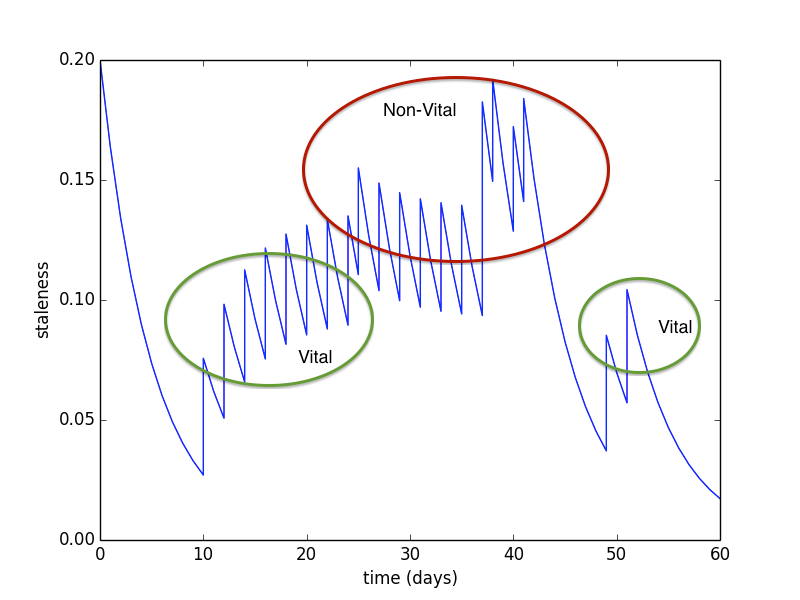
\includegraphics[width=.5\textwidth]{staleness2.png}
\caption{Unkown PhD Student Staleness Example}
\label{stalenesslow}
\end{figure}

Figure \ref{stalenesshigh} intends to represent the exact opposite. It shows an example of an entity with increasing activity in the stream of documents. From $t\mathord{=}10$ we can see that several documents talk about the entity. At first, those documents can be considered vital, but as time goes by and documents continue commenting on the same events, the information starts staling. As an example, let's consider the entity Pearl Jam, a Seattle rock band, which hasn't played in a while. No documents in the stream talk about this entity but when they decide to release their new album, there's a popularity explosion in the stream, which keeps increasing as time passes. At the beginning, releasing a new album can be considered vital information, but after some time, i.e. days, this so-called new information transitions to background information, clearly indicating non-vitalness.

\begin{figure}[h!]
\centering
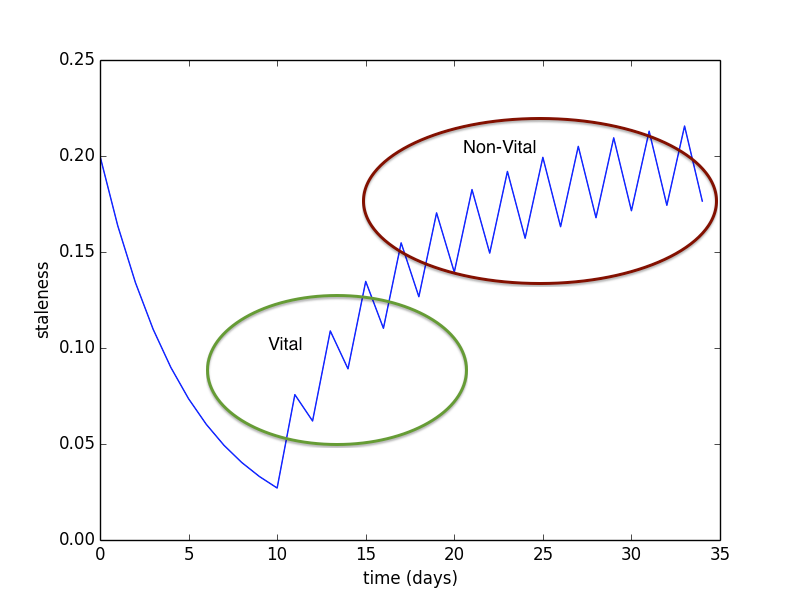
\includegraphics[width=.5\textwidth]{staleness3.png}
\caption{Pearl Jam Staleness Example}
\label{stalenesshigh}
\end{figure}

Finally, Figure \ref{stalenessmedium} aims to represent staleness per topic cluster. We assume that documents about the target entity are assigned to two different topic clusters, $c_1$ and $c_2$. The first main event starts at $t\mathord{=}10$ and continues for a long period of time, showing a growing trend in popularity. The second event starts at $t\mathord{=}50$ and its increasing recognition lasts few days. As an example, let's consider the entity 2014 FIFA World Cup, assume that at $t\mathord{=}10$, the tournament is about to start, and that $c_1$ contains all the documents that talk about the teams that participate. At first, documents talking about the qualified squads can be considered vital information, but after some time, these documents do not drive any update to the entity profile, denoting staleness. Few days after the final, $t\mathord{=}40$, a steep decrease in popularity is shown. At a later time, some documents appear in the stream, and are assigned to $c_2$. They mainly talk about the lessons learned during the competition, denoting vitality.

\begin{figure}[h!]
\centering
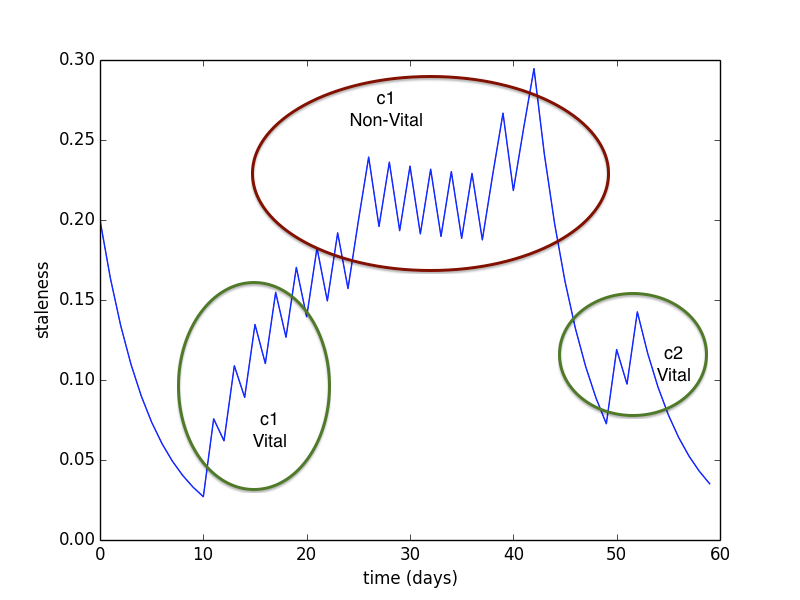
\includegraphics[width=.5\textwidth]{staleness1.png}
\caption{2014 World Cup Staleness Example}
\label{stalenessmedium}
\end{figure}


\subsection{Classifiers}

To apply our method, we propose a multistage classification process with the two classifiers shown below.

\begin{itemize*}
    \item $rnr$: classifies between $referent$ and $non\mathord{-}referent$ documents.
    \item $uv$: discriminates the $referent$ documents into vital or useful subcategories.
\end{itemize*}

Each document goes through the $rnr$ classifier. The $referent$ documents outputted by $rnr$ are used as inputs to the $uv$ model.

\section{Evaluation}
\label{evaluation}

\subsection{Data}

To assess our method we use TRECKBA14 stream corpus. It has around 20M documents annotated with BBN's Serif NLP tools, including within-doc coref and dependency parse trees. Further, we use the 71 target entities given by TRECKBA14 organizers for the Vital Filtering task. Among the 20M documents, around 28K have truth labels. From these, only 8K are training instances while the rest are test examples.

\subsubsection{Preprocess}

We preprocess the corpus to filter the documents that contain exact string matches to the target entities names, including canonical and surface form names.

\subsection{Features}
\label{feat}

A summary of the features used in this paper is presented below. Basic features are borrowed from \cite{jingang13}.

\begin{itemize*}
  \item \textbf{Basic}
    \begin{itemize*}
      \item $Document$
        \begin{itemize*}
            \item $log(length)$: log of document length
            \item $source$: discretized document source
        \end{itemize*}
      \item $Document-Entity$
        \begin{itemize*}
            \item $n(d,e)$: \# of occurrences of the target entity $e$ in document $d$
            \item $n(d,e_p)$: \# of occurrences of partial name of target entity $e$ in document $d$
            \item $fpos(d,e)$: position of first occurrence of entity $e$ in document $d$
            \item $fpos_n(d,e)$: $fpos(d,e)$ normalized by document length
            \item $fpos(d,e_p)$: position of first occurrence of partial name of entity $e$ in document $d$
            \item $fpos_n(d,e_p)$: $fpos(d,e_p)$ normalized by document length
            \item $lpos(d,e)$: position of last occurrence of entity $e$ in document $d$
            \item $lpos_n(d,e)$: $lpos(d,e)$ normalized by document length
            \item $lpos(d,e_p)$: position of last occurrence of partial name of entity $e$ in document $d$
            \item $lpos_n(d,e_p)$: $lpos(d,e_p)$ normalized by document length
            \item $spread(d,e)$: $lpos(d,e) - fpos(d,e)$
            \item $spread_n(d,e)$: $spread(d,e)$ normalized by document length
            \item $spread(d,e_p)$: $lpos(d,e_p)\mathord{-}fpos(d,ep)$
            \item $spread_n(d,e_p)$: $spread(d,e_p)$ normalized by document length
        \end{itemize*}
    \end{itemize*}
  \item \textbf{Embeddings}
    \begin{itemize*}
        \item $v_{d_{i-}}$: mean word embedding of certain part of speech tag in the entity context
    \end{itemize*}
  \item \textbf{Non-parametric Clustering}
    \begin{itemize*}
        \item $min$: minimum distance to existent topic clusters
        \item $avg$: avg distance to existent topic clusters
        \item $zero$: $\mathbbm{1}_{0}{(d_{i-})}$, i.e. flag set to 1 if the word embedding representation of the $i$-th document is $0$
    \end{itemize*}
  \item \textbf{Staleness}
    \begin{itemize*}
        \item $staleness(e)$: staleness of entity $e$, see section \ref{staleness}
        \item $staleness(tc)$: staleness of topic cluster $tc$.
    \end{itemize*}
\end{itemize*}


\subsection{Experiments}

We use two extremely randomized tree ensembles classifiers \cite{GEW06a} in cascade, each composed of 100 weak learners. Each tree in the ensembles has depth 150.

We perform 8 experiments. All of them use the same $rnr$ model trained with the basic features listed in section \ref{feat}.

The different methods differ only on the $uv$ classifier. Explanations of the different $uv$ configurations are detailed below.

\begin{itemize*}
  \item $f\_basic\_single$: baseline method. Uses Basic $Document$ and $Document-Entity$ features.
  \item $f\_basic\_multi$: baseline method. Same as $f\_basic\_single$ but with multitask-learning \cite{Caruana93multitasklearning}.
  \item $f\_emb\_comb$: same as $f\_basic\_multi$ but with Embeddings features computed using the pre-trained Google News dataset. A single combined embedding is calculated from the nouns, proper nouns and verbs found in the entities contexts.
  \item $f\_emb\_pos$: same as $f\_emb\_comb$ but instead of a single combined embedding, it includes one embedding per word type, i.e. one for nouns, one for proper nouns, and one for verbs.
  \item $f\_mean\_stat$: same as $f\_emb\_pos$ but with Staleness and Non-parametric Clustering features, computed per word type. $\alpha = 1$, $\gamma_d = 0$, $\gamma_i = 1$.
  \item $f\_mean\_dyn$: same as $f\_mean\_stat$ but with different hyperparameters. $\alpha = 1$, $\gamma_d = 1$, $\gamma_i = 0.1$.
  \item $f\_clust\_stat$: same as $f\_mean\_stat$ but with different hyperparameters. $\alpha = 0.8$, $\gamma_d = 0$, $\gamma_i = 1$.
  \item $f\_clust\_dyn$: same as $f\_mean\_stat$ but with different hyperparameters. $\alpha = 0.8$, $\gamma_d = 1$, $\gamma_i = 0.1$.
\end{itemize*}

\subsection{Results}

Table \ref{res} shows the micro F1 and SU results of our methods, computed using KBA oficial scorer tool.

\begin{table}[H]
\center
\begin{tabular}{|c|c|c|c|c|} \hline
\textbf{Model} & \textbf{F1} & \textbf{SU} \\ \hline\hline
$f\_basic\_single$ & 0.355 & 0.437 \\ \hline
$f\_basic\_multi$ & 0.492 & 0.520 \\ \hline
$f\_emb\_comb$ & 0.534 & 0.537 \\ \hline
$f\_emb\_pos$ & 0.498 & 0.518 \\ \hline
$f\_mean\_stat$ & 0.520 & 0.532 \\ \hline
$f\_mean\_dyn$ & 0.524 & 0.535 \\ \hline
$f\_clust\_stat$ & 0.527 & 0.537 \\ \hline
$f\_clust\_dyn$ & 0.518 & 0.529 \\ \hline
\end{tabular}
\caption{TRECKBA14 Vital Filtering scores}
\label{res}
\end{table}

As reported in Table \ref{res}, $f\_emb\_comb$ approach is the overall best run on the $vital$ filtering task. Our two baselines ($f\_basic\_single$ and $f\_basic\_multi$) perform as expected. The F1 difference between the two baselines evidences that multitask-learning does work.

All the more advanced runs perform better than both baselines. Using a combined embedding ($f\_emb\_comb$) outperforms using individual embeddings per part of speech tags ($f\_emb\_pos$).

Though the non-parametric clustering and staleness runs perform slightly worse than the simple $f\_emb\_comb$ approach, they illustrate the importance of these new features as they improve the performance of the $f\_emb\_pos$ model.

The worse performance of these more advanced models may be caused by the lack of enough training data. We also believe that exploiting external resources such as Wikipedia entity pages to construct more features, should probably increase the overall accuracy of our method.

It would also be interesting to assess the effects of using different pre-trained word embeddings. We believe that further experimental investigations are needed to account for the correct tunning of the hyperparameters of the model.

\section{Related Work}
\label{related}

Streaming document filtering is related to several fields, including but not limited to, entity linking \cite{KBP11}, text categorization \cite{HLTCOE12}, news surveillance \cite{Steinberger14}.

Several comparative knowledge based population competitions have run in the recent past testifying on the great progress achieved in these fields \cite{gross_doucet_toivonen_trec12}. 

\cite{xitong12} presented one of the best performing systems in TRECKBA12. They created wider representations of entity profiles based on a Wikipedia snapshot and considering the anchor text of all internal Wikipedia links as related entities. In TRECKBA13 competition, different families of methods were proposed, query expansion, classification, learning to rank. 

Our strategy is somewhat similar to \cite{jingang13} in the sense that we first target for a high recall system and then apply different classification methods to differentiate between useful and vital documents. Nevertheless, one key difference is that we do not exploit any external resources to construct features, e.g. we do not use Wikipedia entity pages nor existing citations in the Wikipedia page of an entity, etc. 

Representing words as continuous vectors has been around for a while \cite{Hinton87, Elman90findingstructure}. The progress of machine learning techniques in recent years enabled training more complex models on much larger data sets \cite{mikolovChen}. One popular approach to increase accuracy in existing system is to use unsupervised methods to create word features, or to download word features that have already been produced \cite{Turian10wordrepresentations}. In our method, we do the latter, we use already induced word embedding features in order to improve its accuracy.

To our best knowledge, no recent techniques that combine distributed word embeddings, non-parametric clustering and the staleness notion representations have been proposed to solve this problem.

The closest example we found that addresses the problem of staleness detection is \cite{gamon}, where he builds an association graph connecting sentences and sentence fragments, and uses some graph-based features as good indicators of lack of novelty.

\section{Discussion and Future Work}
\label{related}

A possible line of future reseach would be exploring hierarchical clustering algorithms to better represent topic clusters.

\section{Conclusion}
\label{conclusion}

Filtering streaming documents to accelerate users filling knowledge gaps plays a crucial role in the maintenance and update of knowledge bases.
With the exponential increase of information on the web, it becomes critical to detect relevant documents and incorporate their information to entities in a timely manner \cite{jingang13}.

In this paper we introduce a semi-supervised learning model for document classification tasks. We propose a distributed, non-parametric representation of documents suitable for streaming settings, that groups entity references into topic clusters. Further, we present a notion of staleness computed per entity as well as per topic cluster, which dynamically estimates the entity and cluster relevances.

Combining these three core ideas, distributed word embeddings, non-parametric clustering, and staleness, results in a more accurate representation of entity contexts, and simultaneously addresses the filtering requirements of large corpuses of streaming text documents.

\section*{Acknowledgments} 
 
This work was supported in part by the Argentine Ministry of Science, Technology and Productive Innovation and the TerraSwarm Research Center, supported by the STARnet phase of the Focus Center Research Program (FCRP). Any opinions, findings and conclusions or recommendations expressed in this material are those of the authors and do not necessarily reflect those of the sponsors.

\bibliography{summer_research_paper}
\bibliographystyle{icml2014}

\end{document} 


